\begin{frame}
    \frametitle{Outline}
    \begin{enumerate}
		\item Linear splitting trees
			\begin{itemize}
				\item Upper bounds
				\item Lower bounds for Pigeonhole and 2-fold Tseitin formulas
			\end{itemize}

		\item Proof system Res-Lin 
			\begin{itemize}
				\item Semantic and syntactic version are equivalent
				\item Implication completeness
				\item Simulation in R(lin)
			\end{itemize}

	\end{enumerate}
\end{frame}


\begin{frame}
    \frametitle{Splitting trees}
    $(\lnot x \lor y) \land (x \lor \lnot y) \land (\lnot y \lor z) \land
    	(y \lor \lnot z) \land (x \lor z) \land (\lnot x \lor \lnot z)$ 
	\only<1>{\tikzstyle{end} = [circle, minimum size = 0.1cm, draw, inner sep = 0.1pt]
\tikzstyle{leaf} = [circle, minimum size = 0.6cm, draw, inner sep = 0.1pt, blue]
            
\tikzstyle{level 1}=[level distance = 1.5cm, sibling distance = 3cm]
\tikzstyle{level 2}=[sibling distance = 3cm]
\tikzstyle{level 3}=[sibling distance = 3cm]
    
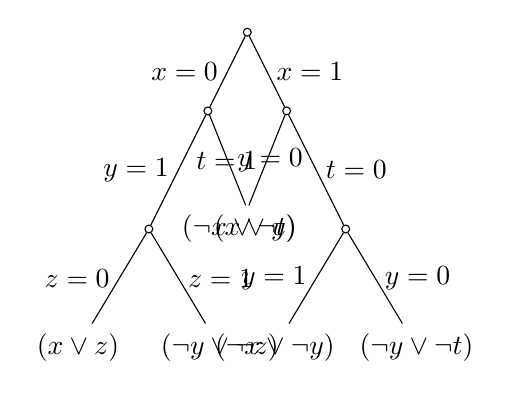
\begin{tikzpicture}[label distance=8mm]
	\node [end] {}
        child {
        	node[end] {}
           	child {
               	node[end] {}
               	child {
                	node {\alert{$(x \lor z)$}}
	                edge from parent
		            node[left] {$z = 0$}
	            }
			    child {
	                node {\alert{$(\neg y \lor \neg z)$}}
	                edge from parent
		            node[right] {$z = 1$}
	            }
                edge from parent
	            node[left] {$y = 1$}
            }
            child[sibling distance = 1.2cm] {
               	node {\alert{$(x \lor y)$}}
                edge from parent
	            node[right] {$y = 0$}
            }
           	edge from parent
            node[left] {$x = 0$}
        }
        child {
        	node[end] {}
            child[sibling distance = 1.2cm] {
            	node {\alert{$(\neg x \lor \neg t)$}}
                edge from parent
                node[left] {$t = 1$}
            }
            child {
            	node[end] {}
                child {
            		node {\alert{$(\neg x \lor \neg y)$}}
	                edge from parent
    	            node[left] {$y = 1$}
        	    }
                child {
            		node {\alert{$(\neg y \lor \neg t)$}}
                	edge from parent
	                node[right] {$y = 0$}
    	        }
                edge from parent
                node[right] {$t = 0$}
            }
           	edge from parent
            node[right] {$x = 1$}
        };
\end{tikzpicture}

%%% Local Variables: 
%%% mode: latex
%%% TeX-master: t
%%% End: 
}
	\only<2>{\tikzstyle{end} = [circle, minimum size = 0.1cm, draw, inner sep = 0.1pt]
\tikzstyle{leaf} = [circle, minimum size = 0.6cm, draw, inner sep = 0.1pt, blue]
            
\tikzstyle{level 1}=[level distance = 1.5cm, sibling distance = 5cm]
\tikzstyle{level 2}=[sibling distance = 4cm]
\tikzstyle{level 3}=[sibling distance = 1.5cm]
    
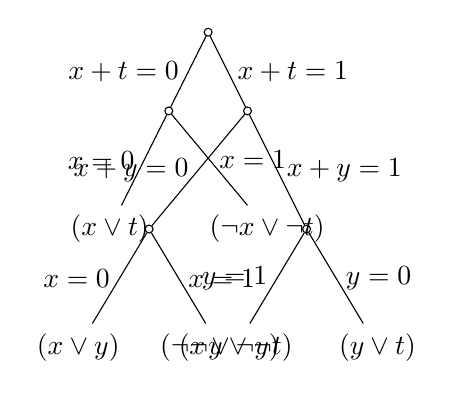
\begin{tikzpicture}[label distance=8mm]
	\node [end] {}
        child {
        	node[end] {}
           	child {
               	node {\alert{$(x \lor t)$}}
                edge from parent
	            node[left] {$x = 0$}
            }
            child[sibling distance = 2.5cm] {
               	node {\alert{$(\neg x \lor \neg t)$}}
                edge from parent
	            node[right] {$x = 1$}
            }
           	edge from parent
            node[left] {$x + t = 0$}
        }
        child {
        	node[end] {}
            child[sibling distance = 2.5cm] {
                node[end] {}
                child {
            		node {\alert{$(x \lor y)$}}
	                edge from parent
    	            node[left] {$x = 0$}
        	    }
                child {
            		node {\alert{$(\neg x  \lor \neg y)$}}
                	edge from parent
	                node[right] {$x = 1$}
    	        }
                edge from parent
                node[left] {$x + y = 0$}
            }
            child {
            	node[end] {}
                child {
            		node {\alert{$(\neg y \lor \neg t)$}}
	                edge from parent
    	            node[left] {$y = 1$}
        	    }
                child {
            		node {\alert{$(y \lor t)$}}
                	edge from parent
	                node[right] {$y = 0$}
    	        }
                edge from parent
                node[right] {$x + y = 1$}
            }
           	edge from parent
            node[right] {$x + t = 1$}
        };
\end{tikzpicture}

%%% Local Variables: 
%%% mode: latex
%%% TeX-master: t
%%% End: 
}
\end{frame}



\begin{frame}
    \frametitle{Linear splitting trees (LST)}
	Solving CNF SAT using splitting by linear forms over $\mathbb{F}_2$
    \begin{columns}
        \begin{column}{3cm}
            Degenerate leaf
            \tikzstyle{end} = [circle, minimum size = 0.1cm, draw, inner sep = 0.1pt]
\tikzstyle{leaf} = [circle, minimum size = 0.6cm, draw, inner sep = 0.1pt, blue]
            
\tikzstyle{level 1}=[level distance = 1cm, sibling distance = 1cm]
\tikzstyle{level 2}=[level distance = 1.5cm, sibling distance = 1.5cm]
\tikzstyle{level 3}=[level distance = 1.5cm, sibling distance = 1.8cm]


    
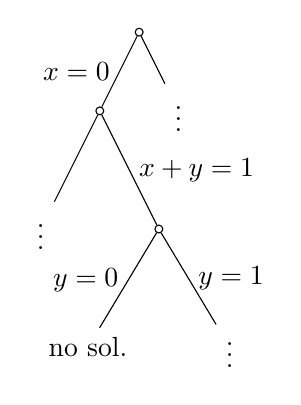
\begin{tikzpicture}[label distance = 8mm]
	\node [end] (z){}
        child {
        	node[end] (b) {}
            child {
    			node {$\vdots$}
		        edge from parent
	    		node[left] {}
			}
		    child {
		        node[end] {}
                child {
                  	node {\alert{no sol.}}
                    edge from parent
                    node[left] {$y = 0$}
                }
                child {
        			node {$\vdots$}
		           	edge from parent
        		    node[right] {$y = 1$}
		        }
	            edge from parent
		        node[right] {$x + y = 1$}
            }
           	edge from parent
            node[left] {$x = 0$}
        }
        child {
        	node (b) {$\vdots$}
           	edge from parent
            node[right] {}
        };
\end{tikzpicture}

%%% Local Variables: 
%%% mode: latex
%%% TeX-master: t
%%% End: 

        \end{column}
        \begin{column}{3cm}
            Sat. assignment
            \tikzstyle{end} = [circle, minimum size = 0.1cm, draw, inner sep = 0.1pt]
\tikzstyle{leaf} = [circle, minimum size = 0.6cm, draw, inner sep = 0.1pt, blue]
            
\tikzstyle{level 1}=[level distance = 1cm, sibling distance = 1cm]
\tikzstyle{level 2}=[level distance = 1.5cm, sibling distance = 1.5cm]
\tikzstyle{level 3}=[level distance = 1.5cm, sibling distance = 1.8cm]


    
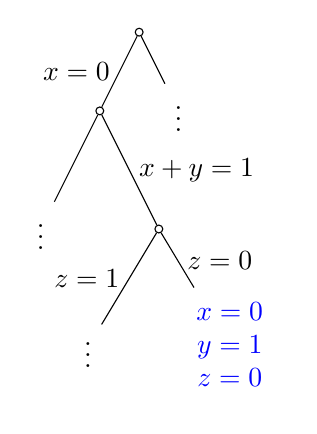
\begin{tikzpicture}[label distance = 8mm]
	\node [end] (z){}
        child {
        	node[end] (b) {}
            child {
    			node {$\vdots$}
		        edge from parent
	    		node[left] {}
			}
		    child {
		        node[end] {}
                child {
        			node {$\vdots$}
		           	edge from parent
        		    node[left] {$z = 1$}
		        }
                child {
                  	node[blue] {\begin{tabular}{c} $x = 0$ \\ $y = 1$ \\ $z = 0$ \end{tabular}}
                    edge from parent
                    node[right] {$z = 0$}
                }
	            edge from parent
		        node[right] {$x + y = 1$}
            }
           	edge from parent
            node[left] {$x = 0$}
        }
        child {
        	node (b) {$\vdots$}
           	edge from parent
            node[right] {}
        };
\end{tikzpicture}

%%% Local Variables: 
%%% mode: latex
%%% TeX-master: t
%%% End: 

        \end{column}
        \begin{column}{3cm}
            Contradiction with a clause
            \tikzstyle{end} = [circle, minimum size = 0.1cm, draw, inner sep = 0.1pt]
\tikzstyle{leaf} = [circle, minimum size = 0.6cm, draw, inner sep = 0.1pt, blue]
            
\tikzstyle{level 1}=[level distance = 1cm, sibling distance = 1cm]
\tikzstyle{level 2}=[level distance = 1.5cm, sibling distance = 1.5cm]
\tikzstyle{level 3}=[level distance = 1.5cm, sibling distance = 1.8cm]


    
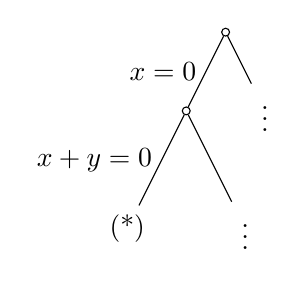
\begin{tikzpicture}[label distance = 8mm]
	\node [end] (z){}
        child {
        	node[end] (b) {}
   		    child {
		        node {\alert{(*)}}
	            edge from parent
		        node[left] {$x + y = 0$}
            }
            child {
    			node {$\vdots$}
		        edge from parent
	    		node[right] {}
			}
           	edge from parent
            node[left] {$x = 0$}
        }
        child {
        	node (b) {$\vdots$}
           	edge from parent
            node[right] {}
        };
\end{tikzpicture}

%%% Local Variables: 
%%% mode: latex
%%% TeX-master: t
%%% End: 

        \end{column}
    \end{columns}
    
	$\Phi$ refutes $(x_1 \lor x_2 \dots \lor x_k)$ iff $\Phi \land (x_i = 1)$ is
    unsatisfiable $\forall i$.
\end{frame}



\begin{frame}
    \frametitle{Algorithm by Seto and Tamaki}

	\begin{itemize}
		\item{} [Seto, Tamaki, 2011] Algorithm for Formula-SAT over the full binary
		    basis. For formulas of size $cn$ the algorithm runs $2^{(1 - \mu_c)n}$,
            where $\mu_c$ is a constant.
		\pitem Splitting over linear combinations.
	\end{itemize}    
\end{frame}